% ------------------------------------------------
%-------------------------------------------------
% Created by Ryan Sharp u1090072
% CSC3600 - Final Report
% Due 25th of October 2019
% ------------------------------------------------
% ------------------------------------------------

% ----- Include ----- %
\documentclass[11pt]{article}
\usepackage{graphicx}
\usepackage{amssymb, amsmath}
\usepackage{multirow}
\usepackage{graphicx, color}
\usepackage{wrapfig}
\usepackage{float}
\usepackage{changepage}

\setlength{\parindent}{0pt}

\begin{document}

% ----- Start Title Page ----- %

    \begin{titlepage}
        \centering
        \vspace {1cm}
        \huge{\textbf{CSC3600 Final Report}} \\ [0.1cm]
        \begin{figure}[ht!]
            \centering
            \def\svgwidth{0.5\columnwidth}
            
\includegraphics[scale={0.20}]{USQ.jpg}
        \end{figure}
        \vspace {0.5cm}
        \Large{By} \\
        \Large{\textbf{USQ Learning Emporium}} \\
        \Large{Richard Dobson, Jesse Hare, James McKeown, Vincent Roberts, Ryan Sharp} \\[0.50cm]
        \Large{Examiner} \\
        \Large{\textbf{Dr. Xiaohui Tao}} \\
        \Large{\textit{Senior Lecturer (Computing) – School of Sciences -
PhD QUT}} \\[0.50cm]
        \Large{Project Supervisor} \\
        \Large{\textbf{Assoc. Prof. Stijn Dekeyser}} \\
        \Large{\textit{Associate Professor (Computing) - School of Sciences - PhD Antwerp}} \\[0.50cm]
        \Large{School of Management and Enterprise} \\[0.50cm]

        \Large{Due: Friday 25th of October 2019}
    \end{titlepage}


\newpage

% ----- End Title Page ----- %



% ----- start ToC ----- %

\tableofcontents
\newpage

% ----- start ToC ----- %





\setcounter{secnumdepth}{0}
% ----- Section 1 ----- %

\section{1. Executive Summary}
Over the past three months, USQ Learning Emporium has worked on the file metadata harvester and searcher project. This project required the team to complete the following two objectives:

\begin{enumerate}
\item Develop a CLI script that takes a directory path as input, and returns a CSV-formatted text having one line per file in the directory, and listing all metadata attributes and values extracted from that file.
\item Develop a GUI that reads the above CSV file and displays a spreadsheet-like grid, where rows can be sorted filtered on attribute values, files can be searched for on multiple criteria and double-clicking a file-row opens it.
\end{enumerate}

This report outlines the overall process the team went through to complete the project. This included what methodology the team used, the structure and organisation of the team, the overall outcome of the project, the cost of the project, how professionalism was adhered to and the distribution of tasks between team members. \\

It is the aim of this report to gain further funding for the expansion of the project. This funding will allow the team to add further functionality and provide extensive performance upgrades to the program. It is the opinion of this report that the project was completed to a high standard and that all criteria provided by the client has been met. \\

The report found the following key points in relation to the overall process of the project: 

\begin{itemize}
\item The scrum implementation of the agile methodology was used to complete the project.
\item The 5 person team was divided into two sub-teams, front-end (2 members) and back-end (3 members).
\item Slack, Facebook Messenger and Zoom Video Conferencing were all used for communication between members.
\item The project was delivered successfully, with working versions of the front-end and back-end submitted.
\item The project cost came to a total of, AUD \$8,444
\item Professionalism was kept to a high standard throughout the project duration.
\item Tasks were efficiently distributed between members
\end{itemize}

It is the recommendation of this report that the client continues to work with the USQ Learning Emporium to develop a high quality, highly optimised and complete version of the product. This continued relationship will enable the team to expand staff members and put more resources into developing the final product.


\newpage



% ----- Section 2 ----- %

\section{2. Methodology}

\subsection{2.1 Methodology Statement}
The team used the scrum implementation of the agile methodology to complete the project. The scrum process allowed the team to incrementally build the program over the entire project duration. As there was constant input from the the project supervisor and the client, the scrum process permitted the team to make quick changes.

\subsection{2.2 Justifications}
The following sub sections will describe why scrum was chosen, the benefits of scrum and the disadvantages of scrum.

\begin{adjustwidth}{1cm}{}

\subsubsection{2.2.1 Why Scrum Was Used}
As stated in the previous section, scrum was ideal for this project as it allowed the team to make quick changes during the development process. Another reason why scrum was chosen was because there was no team leader. This provided an environment where all team members could be equal and address issues as a whole group. 

\subsubsection{2.2.2 Benefits of Scrum}
Scrum provided a framework that allowed the team to build in sprints, which suited this type of project. After each sprint, a meeting with the project supervisor was organised so that feedback could be given in preparation for the next sprint. In addition to this, scrum forced the team to prioritise requirements which allowed for faster development. Without this, lower-priority requirements may have been implemented at the cost of the higher-priority requirements.

\subsubsection{2.2.3 Disadvantages of Scrum}
As time constraints were a major factor in the development of the project, it was difficult for the team to have as many daily meetings as scrum required. Scrum requires the implementation of daily meetings, which wasn't feasible with this project. Another disadvantage with scrum in the team's case, was that each member of the team wasn't experienced with the process and the roles involved. This meant that the roles outlined in the scrum process weren't followed 100\% correctly.

\end{adjustwidth}

\subsection{2.3 Discussions}
The following sub sections will discuss how the scrum process was utilised and how it will be used for future projects.

\begin{adjustwidth}{1cm}{}

\subsubsection{2.3.1 How Scrum Was Followed}
All team members simulated the \textit{Product Owner} and \textit{Scrum Master} roles. Due to the inexperience with scrum, it was decided that this was the best option to follow. Daily meetings were reduced to at least 1 meeting a week, with 2 meetings a week the average throughout the duration of the project. Sprints were carried out every 1 to 3 weeks, depending on the size of the individual tasks. Once a sprint was complete a whole team meeting was organised to discuss the next sprint. Meetings were then held with the project supervisor to demonstrate what had been completed and to gain new requirements for the project. 

\subsubsection{2.3.2 How Scrum Will Be Used In The Future}
The obvious improvement to the scrum process in future projects would be to have a dedicated product owner and scrum master. These two roles play a key part in the scrum process, and when included, make the development of the project a lot easier. In addition, having more time to have daily meetings would help tremendously in both planning and developing the project. \\

Due to this being the first time each member had used the scrum process, it can be presumed that it wasn't as efficient as it could have been. As with all projects of this nature, the more experience you have, the faster and more efficient you get. It is the goal of all members, that with each time they use the scrum process they get more proficient with using it.

\end{adjustwidth}


% ----- Section 3 ----- %

\section{3. Project Process}

\subsection{3.1 Team Organisation}
There were a total of 5 members in the USQ Learning Emporium team. As this project was initially designed for teams of 3, the team needed to strategise ways in which to divide the work evenly between members. The first solution was to divide the main project task into 2 sub teams; a back-end team (3 members) and a front-end team (2 members). Within these teams each member had different roles. \\

From these sub teams, each had their own Facebook Messenger group and their own Slack channel for discussing specific project tasks. This stopped unnecessary information from being communicated between the sub teams, i.e. the back-end team didn't need to know the specifics of the front-end and vice versa. Within these messenger platforms, jobs were distributed and agreed upon between members.

\subsection{3.2 Team Structure and Roles}
As stated above, the group was divided into 2 main groups;  a back-end team (3 members) and a front-end team (2 members). The back-end team consisted of: James McKeown (Team Leader), Richard Dobson (Programmer) and Vincent Roberts (Programmer). The front-end team consisted of: Jesse Hare (Team Leader), Ryan Sharp (Programmer). \\

James McKeown and Jesse Hare both lead their respective teams. This allowed for better and more effective team co-ordination. It helped all members stay on task and stopped individual team members from deviating from the plan and doing their own work. Both of these members (James and Jesse) took on the most technical aspects of the project, especially in regards to the planning the project (in terms of coding). Other members then utilised this research to program their respective tasks within the project. 


\subsection{3.3 Communication and Meetings}
The following sub sections will discuss how well the team communicated throughout the project duration.

\begin{adjustwidth}{1cm}{}

\subsubsection{3.3.1 Effectiveness of Communication}
Communication between members was very quick and effective. The team decided to use a private Facebook Messenger chat as the primary point of contact as each member regularly used this application. This made it easier to notify team members of urgent matters. In addition to Facebook, the team decided to use a Slack channel for more technical and project specific subjects. Slack was new to all members and was therefore not utilised to it's full potential. \\

The main problem faced with the Facebook Messenger chat, was that the information couldn't be organised. It would have been better to use Slack as the primary messenger application as it was more suited to this type of project; especially because the project had 5 team members and 2 sub teams. In future projects organisation of information needs to be a higher priority.

\subsubsection{3.3.2 Team Meetings}
Team meetings were run through the Zoom video conferencing application. At least once a week the whole team would meet to discuss the progress of the project. Meetings for the back end and front end team were often held more than once a week to discuss new ideas for their respective tasks. These meetings were highly effective as each member could screen share what they were working on and clearly communicate that with the team. \\

These meetings could be improved by having a set agenda before each meeting. Occasionally the meetings started slow as individual team members all had to organise what they were going to discuss. It would also be ideal to have one member as the designated scribe to take notes for each meeting and relay this back to the team.

\end{adjustwidth}

\subsection{3.4 Documentation}
The activity log sheets, task summary sheets and meeting minute documents all assisted in tracking how the project was developing. The activity log sheets provided a good point of reference each week in deciding what tasks needed to be worked on next. It also helped ensure that each task was completed. Without the activity log sheets and task summaries it would have been difficult to keep track of the progress of the project. However, it was often the case that some weeks would be forgotten and team members would need to go back and fill in the information. This was obviously not ideal, but did not have a noticeable effect on the productivity of the team. \\

The meeting minutes documents were essential for the project. Without them, members of the team would forget what was discussed in each meeting. This would result in a massive amount of lost time as information would need to be repeated. After each meeting with the project supervisor (Stijn Dekeyser), the team would stay back and document what had been discussed in these meetings. This helped tremendously when working on specific parts of the project. This is because the team now had a reference to look at, to see if certain features needed to be implemented. These meeting minutes can be found attached to the bottom of this document.


\subsection{3.5 Process}
The following sub sections will discuss the process used to develop the project, the difficulties encountered with this process and beneficial strategies used throughout the project duration.

\begin{adjustwidth}{1cm}{}

\subsubsection{3.5.1 Overall Process}
The team (and it's sub teams) decided on using the agile methodology for the project. Each week a meeting was held between members to discuss what tasks needed to be completed that week. Every 2 - 3 weeks a meeting was held with the project supervisor to discuss improvements that needed to be made. These improvements (as tasks) were added to the list of tasks to be completed.

\subsubsection{3.5.2 Difficulties Encountered}
Due to time constraints, university commitments and conflicting schedules, some weeks were more challenging than others. As a result some tasks did not get completed on schedule. This resulted in the rescheduling of tasks which hindered productivity. Any difficulty faced was getting team members  schedules to align. Occasionally, tasks would get worked on individually and passed on to another team member. Ideally in the real world, each member would have this project as their number one priority with no external distractions (such as university commitments, work etc.).

\subsubsection{3.5.3 Beneficial Strategies}
Weekly video conference meetings were essential for the project completion. These meetings allowed each member to discuss, and show, exactly what they were working on. Especially as the group implemented the agile methodology, it was important to discuss any improvements to the project each week. \\

Using Trello boards also assisted in the development of the project. It allowed all of the tasks to be laid out for each member to see. Once a task was completed it was moved from the 'to-do' card into the 'completed' card. As there were 5 members of the team, it was extremely beneficial as the tasks could be marked as 'to-do', 'doing' and 'completed'. This helped in reducing and avoiding work that would otherwise be repeated.

\end{adjustwidth}


% ----- Section 4 ----- %

\section{4. Project Report}
\subsection{4.1 Project Outcome}
The following sub sections will discuss the final outcomes of the project.

\begin{adjustwidth}{1cm}{}

\subsubsection{4.1.1 The Project}
The aim of this project was to implement a software solution for the client’s need to search for and examine file metadata from a potentially large dataset. In order to do this, the team had to design and develop a solution that consisted of two components. The first of the two, the file metadata harvester, is used to gather the file metadata from files. The second component, the searcher, makes use of a GUI to display that harvested information. This enables the client to interact with the program, and perform a variety of functions that will aid in their search for particular files.

\subsubsection{4.1.2 Project Outcome} 
The deliverable for the client at the end of this project consisted of two software components, and their supporting documentation. The team has successfully managed to produce working versions of both components. The report will now go over the outcomes for each of these components in more detail.

\subsubsection{4.1.3 Metadata Harvester Outcomes}
The metadata harvester program the back-end team developed can be used to search a specified directory, either recursively or non-recursively, and extract the metadata for any files found within the search area. A recursive search will begin in the target directory, then expand to subdirectories within the current search directory and continue until there are no more subdirectories to search within. If the user specifies that a recursive search is to be performed, it can be expected to take additional time compared to a search performed on a single directory. \\

When the metadata harvester program is invoked and before it’s runtime is over, it will write all the file metadata to a user-specified file. This file is what is used by the searcher program as input to display the file metadata in a more accessible and interactive GUI format. \\

The harvester program extracts metadata using the following methods:

\begin{itemize}
\item \textbf{Hachoir external Python Library} – This tool is the most valuable in regard to metadata extraction, it is able to extract data from a large range of file types, however it still comes with quirks and its own set of challenges
\item \textbf{PyPDF2 external Python Library} – This library is used to extract metadata from PDF files. The team had to use this library because Hachoir deals with most file types except text-based ones, such as pdf, docx, .txt etc. 
\item \textbf{Os Python module} – This useful module native to Python is invaluable in gathering standardised file metadata such as type, creation, modification and accessed dates. This module can extract the same set of data from any type of file, so the team used this module to ensure all files represented in the searcher GUI have at least this subset of metadata information available to the user.

\end{itemize}
	
There are some filetypes in which the data extracted was slightly lacking. Unfortunately, due to time constraints, the team didn't have the time to find more metadata extraction libraries that were focused towards files that the team had difficulty obtaining data for. \\

If the project does get continued funding, the priority for this component will be the broadening of the types of metadata that can be extracted from a larger range of filetypes. This is not a difficult task, however, it is time consuming as all metadata extraction libraries extract their data in different ways. For the software to work the team needs it all in the standardised CSV format when output to a file. \\

The team is confident that the client will be satisfied with this portion of the project deliverable. This is because they have indicated that their main intentions were to harvest data from their own personal files. The types of  files they will be harvesting are for the most part supported by the metadata harvester program. \\

It is worth noting, that as could be expected, the harvesting operation can take additional time when harvesting a high volume of files. Although some optimisation was attempted, the team is of the opinion that they could reduce the wait time for users when running the program. \\

In summary, the team is of the opinion that the harvester metadata program meets the client’s requirements. However, there is room for improvement in regard to performance and the range of files from which unique metadata is gathered. This will be addressed should the project gets continued funding.


\subsubsection{4.1.4 Metadata Searcher Outcomes}
The fundamental aim of the metadata searcher program was to develop a GUI that displayed the harvested file metadata. This metadata could be interacted in a way that would facilitate sorting/searching and filtering on file metadata values to enable a user to locate certain files or groups of files that share common attributes easily. \\

This aim was achieved quite early on, however over the course of development, there were additional requirements introduced that improved the searcher programs usability and utility. The GUI design and layout itself changed multiple times over the development process, as well as the functionality and usage of GUI elements. \\

The front-end team decided to make use of the external Python library PyQt5 to handle the GUI implementation, but all other libraries used were modules that were native to Python. The most important module the team used besides PyQt5, was the SQLite3 library. This library enables the creation of Relational Databases using the Structured Query Language. This proved invaluable in storing the harvested metadata, especially interacting with it through SQL queries. This enabled the team to manipulate and interact with that data in many ways, opening a lot of possibilities regarding the searcher programs functionality. \\

In the end the team ended up meeting all critical and non-critical requirements gathered from the client over the course of development. The functionalities that the searcher program provides for the client includes:

\begin{itemize}
\item Sorting/Searching of Metadata based on one or more fields
\item Ability to open files when clicking on the filepath in their respective record
\item Filtering of results based on one or more fields
\item Responsiveness
\item Ease of Use
\end{itemize}

Although the team is confident that this component has met the client’s expectations, they realise that there is always room for improvement. Further development on the searcher program will likely be focused toward performance improvements, and possibly even additional functionality such as deletion and renaming of files, which could prove to be of great utility for the client. \\

Although the team dedicated a lot of resources towards performance and optimisation, the user should still expect that the searcher program may take some time to gather and collect metadata from large csv files. Once the GUI has launched however, all subsequent operations can be expected to perform without delay. The reason for this is that operations on a Relational Database using SQL tend to be quite efficient. \\

The team is thoroughly satisfied with what they have developed regarding the searcher program, and they hope the client feels the same way. They are confident that it has met all of the client's needs and expectations. The team hopes that it remains an important utility for the client for the foreseeable future.

\end{adjustwidth}

\subsection{4.2 Project Quality}
The following sub sections will discuss the quality of the final project submission.

\begin{adjustwidth}{1cm}{}

\subsubsection{4.2.1 Usability}
Regarding the harvesting of metadata, using the harvester program is simple. To harvest metadata from a directory, the user simply needs to provide the harvester script - the ‘-r’ option - if they wish to harvest from a directory recursively, and the path to the output file. If the user enters the arguments incorrectly a help dialog will print to the screen instructing them on the correct command to execute the harvester program from the CLI. Once executed, the user simply must wait briefly until the harvester program has been executed. \\

With the Searcher program, execution is even simpler from the CLI. All that is required for an argument is the csv file produced by the harvester program. After a brief wait, the GUI appears on screen. Most of the elements are accompanied by labels, and tooltips on mouseover, and those that aren’t resemble constructs seen in many other types of applications, following common conventions in relation to GUI design. Examples of the intuitive features are things such as double clicking on a column header to sort, and the results filter that appears above the displayed metadata. The only part of the GUI where a user may get caught out or feel unsure, will provide information on incorrect user input that instructs the user on the correct way of using that widget. Another intuitive feature the team included is the ability to double click on file paths to open the file, which is a common practice in many file manager/explorer applications, and it is something that most users may try to do automatically. \\

\subsubsection{4.2.2 Completeness}
As far as the harvester program is concerned, all requirements have been met, and it performs as it should. That being said, there is always the opportunity to expand on the range of filetypes that the harvester program can extract metadata from, as well as the range of potential metadata types it can extract. \\

The searcher program has met all requirements as well, functional and non-functional. As new requirements are introduced, the team added them promptly, and if development continues so will the addition of features to the searcher program.

\subsubsection{4.2.3 Maintainability}
As far as maintainability is concerned, that only concerns the harvester program. Maintenance may include the adding/removal/updating of the libraries used to collect the file metadata, but in the end as long as the output remains in the same format, there should be no changes needed on the GUI side of things. Also, there is a generous amount of commenting throughout both the searcher and harvester programs, so developers not familiar with the project would easily be understand how the code works and how to modify it if needed.

\subsubsection{4.2.4 Reliability}
Reliability issues have been found only in a couple of isolated cases. For the harvester program, data that is not usable by the searcher program or meaningless to a user may be harvested if the harvester is executed on any sort of system folders. The reason being that these folders can sometimes contain obscure filetypes which often have no readable metadata, or the metadata that is read is either of no use to detrimental to the program’s operation. \\

As far as the searcher program is concerned, as long as the input csv file is in the correct format, there should be no issues. The searcher program has been thoroughly tested and there has been a significant amount of bug removal to ensure as stable of a user experience as possible.

\subsubsection{4.2.5 Portability}
Both programs have been designed to work on Linux. Early in development however, the team had working versions on windows as well, so If needed further down the track cross-compatibility implementation would not be too big of an issue. As long as the user has python 3.7.x, the Hachoir, PyPDF2 and PyQt5 libraries installed, they should be able to use these programs on any Linux distros.

\subsubsection{4.2.6 Performance}
Time from execution to completion of the Harvester program is linearly related with the number of files to harvest metadata from. The more files that are harvested for metadata, the longer it will take. Harvesting using a recursive search of approximately 3500 files will take around 2minutes on a mid-range laptop. \\

The time from execution to display of the searcher GUI takes slightly more time, however, once the GUI is loaded most if not all operations are near instant. It is important to us that the user is aware of potential waiting times.

\end{adjustwidth}

\subsection{4.3 Cost of the Project}
The following sub sections will discuss the time and labor costs of the project.

\begin{adjustwidth}{1cm}{}

\subsubsection{4.3.1 Cost of Hardware}
There are no deviations to the cost of hardware from the projection provided in the initial project plan. The costing table can be viewed below. \\

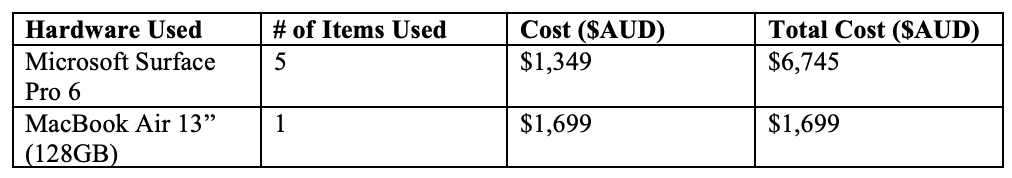
\includegraphics[scale=0.71]{hardware_table.png} \\

As the project was worked on remotely, all team members required company issued equipment. There were a total of 5 Windows machines provided to each member, with an additional MacBook Air provided to the project leader, James McKeown. There were no unexpected circumstances that required the purchase of any other pieces of hardware.

\subsubsection{4.3.2 Cost of Software}
There were multiple software solutions that were incorporated for the development of the project. There were some software solutions that were not foreseen in the initial project plan. All of the software solutions can be viewed below. \\

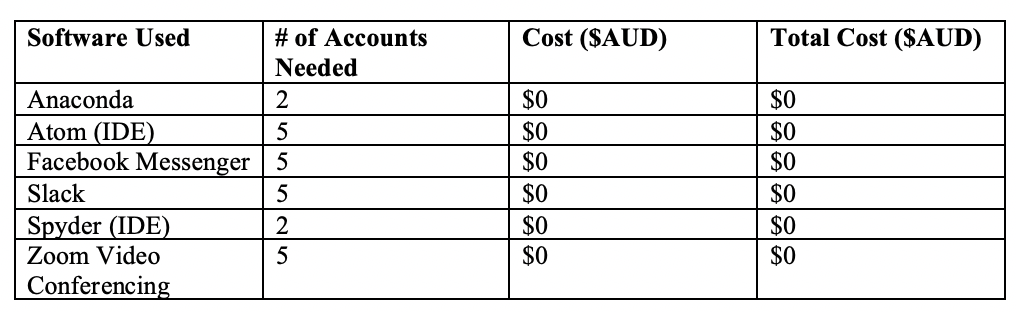
\includegraphics[scale=0.71]{software_table.png} \\

In the planning stages it was decided the front-end team would use Spyder as the preferred IDE. It added more specific functionality compared to Atom in this case. Anaconda was also used for the development of the front-end GUI. Facebook Messenger and Slack were used for communication between team members. Zoom Video Conferencing was used for group meetings and screen sharing. \\

\subsubsection{4.3.3 Time Cost}
The project took 12 weeks to complete with each member contributing 20 hours a week. Each member therefore contributed 240 hours of work to the project with a combined team total of 1,200 hours.

\subsubsection{4.3.4 Labor Cost}
The team was split up into 2 sub teams, a front-end team and a back-end team. The front-end team consisted of Jesse Hare and Ryan Sharp. The front-end team consisted of James McKeown, Richard Dobson and Vincent Roberts. \\

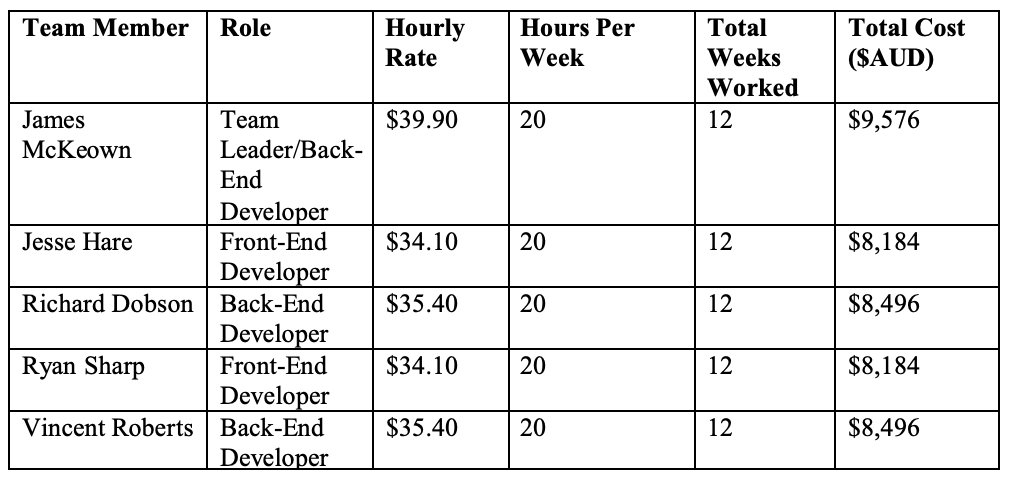
\includegraphics[scale=0.71]{team_cost.png} \\

The only difference between the projected labor cost and the actual labor cost was the error in how many weeks the project would take. It was initially predicated that the project would run over 10 weeks, when in fact the project ran for a total of 12 weeks.

\subsubsection{4.3.5 Lessons Learnt About Project Cost Estimation}
The major lesson learnt was that no prediction about the cost will be 100\% accurate. Lots of things change in a 12 week period and there is no possible way that these can be accounted for. For example, majority of team members used Atom before this project, so it was assumed that the team would use this again. However, once the front-end team researched more into what programs were out there, it was decided that Atom was not the idea choice and that the team should use Spyder instead. \\

\end{adjustwidth}

% ----- Section 5 ----- %

\section{5. Professionalism and Professional Ethics}

\subsection{5.1 Professionalism}
Throughout the project, professionalism was kept to a relatively high standard. In future projects, it would be optimal to have a set of professional standards that outlines what is 	expected of each team member. This would allow the team to refer back to this document should any breach of the standards occur. The following sub sections will discuss issues related to professionalism that occurred during the project.\\

\begin{adjustwidth}{1cm}{}

\subsubsection{5.1.1 Client Interaction Confusion}
Client interaction is the most important part of a project, without them the project would not exist. In this project, the client was also the project supervisor who gave information on behalf of both parties. While this did not have a major effect on the outcome of the project, it was obviously difficult to differentiate between a client meeting and project supervisor meeting. As a team, we should have been clearer with the meetings we wanted to have. Upon reflection, it would have been better if we clearly communicated they type of meeting we would like with the project supervisor. 

\subsubsection{5.1.2 Lack of Client Interaction}
It is important for any project to get as much client input as possible too ensure client satisfaction. While the team met the required amount of meetings with the client, it was most likely not enough. In a real world scenario it would have been best to meet with the client every 1 to 2 weeks, especially as the scrum process was used. This would have ensured that at every sprint the client had some input into the project and could see updates regularly. 

\subsubsection{5.1.3 Team Communication}
Communication between team members is essential for the progress of a project. On occasion, some team members did not reply to messages in a timely manner. This effected the progress of the project as some work had to be delayed to due other work not being completed. This was addressed via a team meeting, where all members gave their opinions on the matter. The issue was addressed and after the meeting took place, this particular issue did not happen again.

\end{adjustwidth}

\subsection{5.2 Professional Ethics}
Throughout the project professional ethics was also kept to a relatively high standard. As this project was conducted in a university environment, and was therefore a mock real world project, there was only one major professional ethic concern. This will be discussed in the following sub section.

\begin{adjustwidth}{1cm}{}

\subsubsection{5.2.1 Sharing of Sensitive Client Information}
Data privacy should be top priority for any business and associated business project. Due to financial constraints of the project is was not feasible to have a private GitHub repository. This resulted in the team using a public GitHub repository that could be accessed by any member of the public. In a real world scenario this would obviously be very bad practice. In future projects, with more financial backing, it would be essential that a private GitHub repository be used. \\

\end{adjustwidth}


% ----- Section 6 ----- %

\section{6. Contribution Distribution}

\subsection{6.1 How Work Was Distributed}
Each sub team, front-end and back-end, were responsible for their own individual tasks. Meetings were held on a weekly basis to decide what tasks needed to be completed that specific week. These tasks were allocated to team members based on their previous knowledge and experience of the task. For example, Jesse had previous experience with some Python GUI elements, so he was tasked with researching and developing the initial concept.


\subsection{6.2 How Effective Was The Distribution}
This method of distributing tasks worked quite well and resulted in a clear structure that needed to be followed. Without this distribution, team members would be going off and doing there own thing. This way each member knew exactly what they needed to do. While distributing tasks, there was no way to make sure everyone received the same amount of work. This was the only hurdle faced, but was mitigated as best best as possible.

\subsection{6.3 Task Distribution Table}
The following table represents the tasks completed in the project and the percentage of effort put it in by each team member. \\

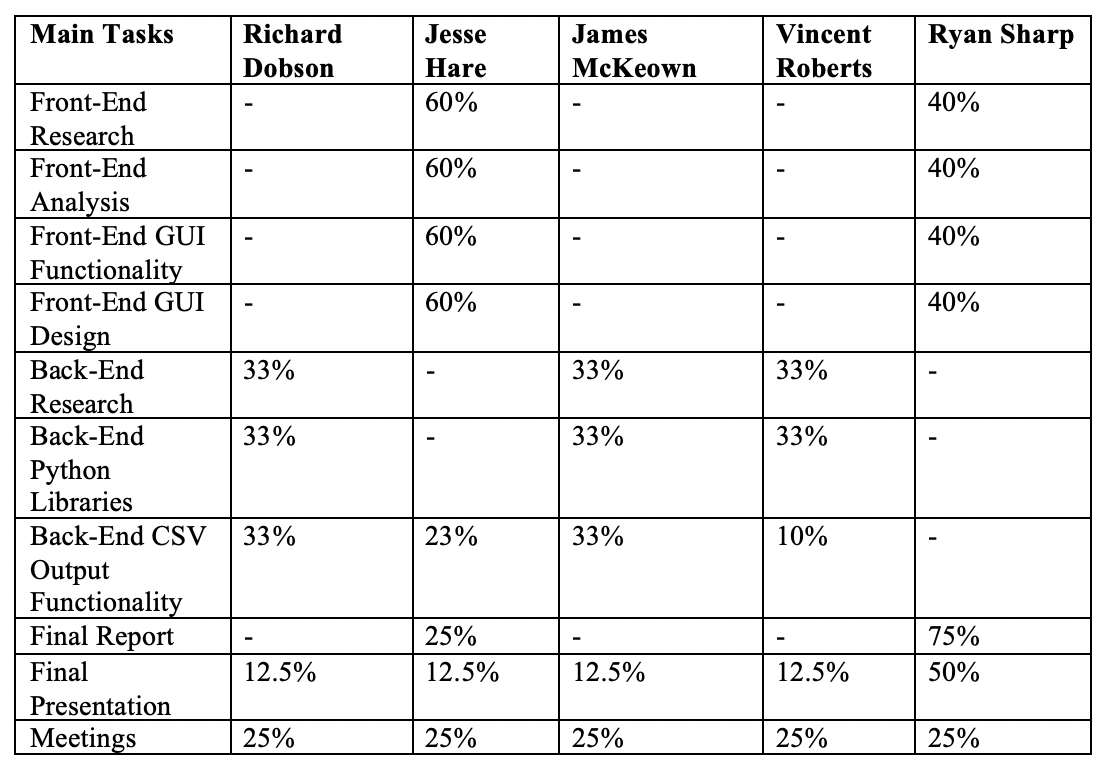
\includegraphics[scale=0.7]{task_distro.png} \\

\newpage


% ----- Section 7 ----- %

\section{7. Conclusions}
This report has outlined the overall process the USQ Learning Emporium team went through to complete the project. This included what methodology the team used, the structure and organisation of the team, the overall outcome of the project, the cost of the project, how professionalism was adhered to and the distribution of tasks between team members. \\

Overall, the team has found this project to be a valuable learning experience in preparation for real world projects. Teamwork is a key skill for real world projects and the team has learned how to work together as a group to complete tasks effectively. A major lesson learnt, was dividing the work into two sub teams, this helped each member focus on their respective tasks and reduced time wasting. \\

As communicated via the report, the team feels there are some key strategies that need to be put in place for future projects.

\begin{enumerate}
\item \textit{Dedicated Slack Channel} - A Slack channel should be used for future projects to keep all project related discussions in one place.
\item \textit{Set Dates For Meetings} - Meetings should be prioritised at the start of each week. These meetings should be held at a minimum of a weekly basis.
\item \textit{Accountability For Lack Of Communication} - There should be a set of standards in relation to communication between team members. Not replying to messages was an issue raised during the project.
\end{enumerate} 

The report found the following key points in relation to the overall process of the project: 

\begin{itemize}
\item The scrum implementation of the agile methodology was used to complete the project.
\item The 5 person team was divided into two sub-teams, front-end (2 members) and back-end (3 members).
\item Slack, Facebook Messenger and Zoom Video Conferencing were all used for communication between members.
\item The project was delivered successfully, with working versions of the front-end and back-end submitted.
\item The project cost came to a total of, AUD \$8,444
\item Professionalism was kept to a high standard throughout the project duration.
\item Tasks were efficiently distributed between members
\end{itemize}

It is the recommendation of this report that the client continues to work with the USQ Learning Emporium to develop a high quality, highly optimised and complete version of the product. This continued relationship will enable the team to expand staff members and put more resources into developing the final product.


\newpage

% ----- Section: Reference List ----- %

\section{Reference List}


\newpage

% ----- Section: Appendix ----- %

\section{Appendix}
1. Overall Project/Time Cost \\
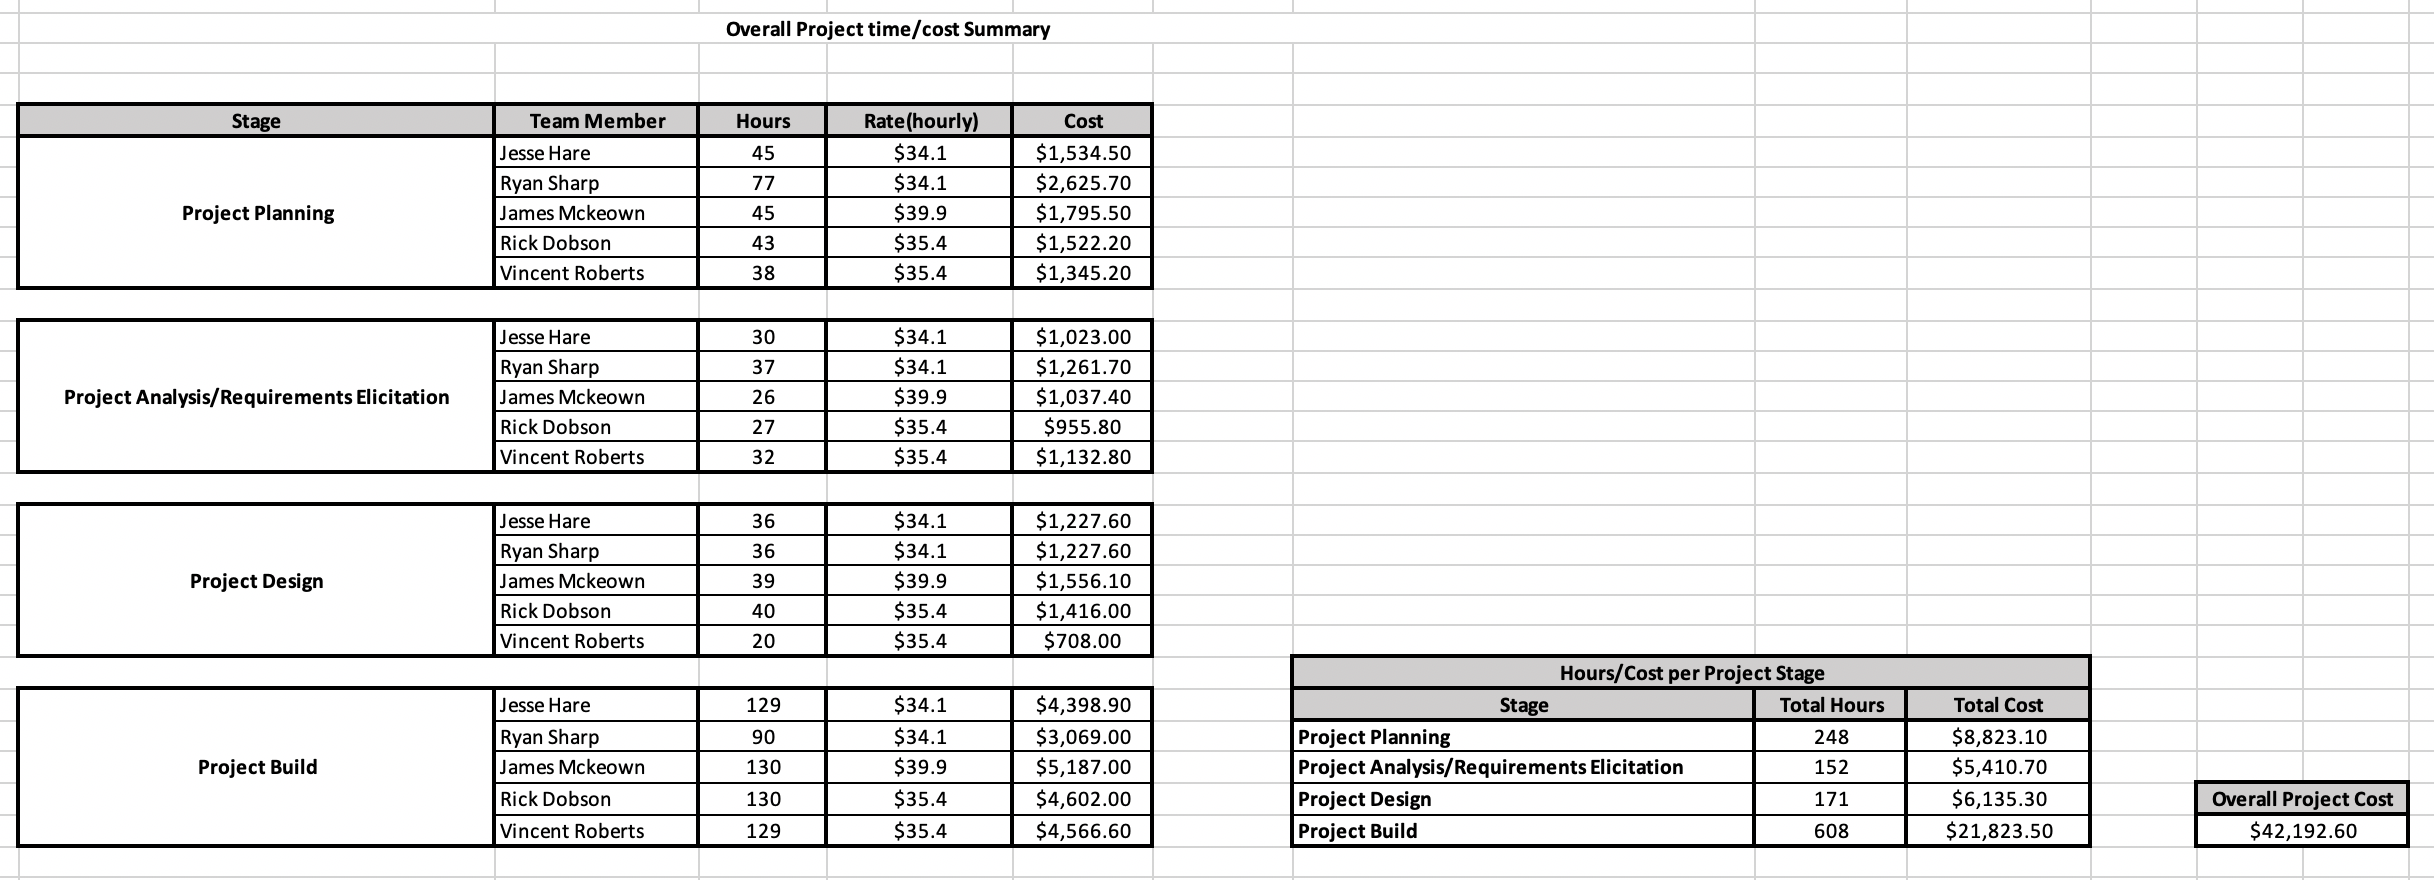
\includegraphics[scale=0.35]{overall.png} \\

Please find attached all other items in the zip folder provided with submission.


\end{document}

